\documentclass[11pt,compress,t,notes=noshow, xcolor=table]{beamer}
\usepackage[]{graphicx}\usepackage[]{color}
% maxwidth is the original width if it is less than linewidth
% otherwise use linewidth (to make sure the graphics do not exceed the margin)
\makeatletter
\def\maxwidth{ %
  \ifdim\Gin@nat@width>\linewidth
    \linewidth
  \else
    \Gin@nat@width
  \fi
}
\makeatother

\definecolor{fgcolor}{rgb}{0.345, 0.345, 0.345}
\newcommand{\hlnum}[1]{\textcolor[rgb]{0.686,0.059,0.569}{#1}}%
\newcommand{\hlstr}[1]{\textcolor[rgb]{0.192,0.494,0.8}{#1}}%
\newcommand{\hlcom}[1]{\textcolor[rgb]{0.678,0.584,0.686}{\textit{#1}}}%
\newcommand{\hlopt}[1]{\textcolor[rgb]{0,0,0}{#1}}%
\newcommand{\hlstd}[1]{\textcolor[rgb]{0.345,0.345,0.345}{#1}}%
\newcommand{\hlkwa}[1]{\textcolor[rgb]{0.161,0.373,0.58}{\textbf{#1}}}%
\newcommand{\hlkwb}[1]{\textcolor[rgb]{0.69,0.353,0.396}{#1}}%
\newcommand{\hlkwc}[1]{\textcolor[rgb]{0.333,0.667,0.333}{#1}}%
\newcommand{\hlkwd}[1]{\textcolor[rgb]{0.737,0.353,0.396}{\textbf{#1}}}%
\let\hlipl\hlkwb

\usepackage{framed}
\makeatletter
\newenvironment{kframe}{%
 \def\at@end@of@kframe{}%
 \ifinner\ifhmode%
  \def\at@end@of@kframe{\end{minipage}}%
  \begin{minipage}{\columnwidth}%
 \fi\fi%
 \def\FrameCommand##1{\hskip\@totalleftmargin \hskip-\fboxsep
 \colorbox{shadecolor}{##1}\hskip-\fboxsep
     % There is no \\@totalrightmargin, so:
     \hskip-\linewidth \hskip-\@totalleftmargin \hskip\columnwidth}%
 \MakeFramed {\advance\hsize-\width
   \@totalleftmargin\z@ \linewidth\hsize
   \@setminipage}}%
 {\par\unskip\endMakeFramed%
 \at@end@of@kframe}
\makeatother

\definecolor{shadecolor}{rgb}{.97, .97, .97}
\definecolor{messagecolor}{rgb}{0, 0, 0}
\definecolor{warningcolor}{rgb}{1, 0, 1}
\definecolor{errorcolor}{rgb}{1, 0, 0}
\newenvironment{knitrout}{}{} % an empty environment to be redefined in TeX

\usepackage{alltt}
\newcommand{\SweaveOpts}[1]{}  % do not interfere with LaTeX
\newcommand{\SweaveInput}[1]{} % because they are not real TeX commands
\newcommand{\Sexpr}[1]{}       % will only be parsed by R



\usepackage[english]{babel}
\usepackage[utf8]{inputenc}

\usepackage{dsfont}
\usepackage{verbatim}
\usepackage{amsmath}
\usepackage{amsfonts}
\usepackage{bm}
\usepackage{csquotes}
\usepackage{multirow}
\usepackage{longtable}
\usepackage{booktabs}
\usepackage{enumerate}
\usepackage[absolute,overlay]{textpos}
\usepackage{psfrag}
\usepackage{algorithm}
\usepackage{algpseudocode}
\usepackage{eqnarray}
\usepackage{arydshln}
\usepackage{tabularx}
\usepackage{placeins}
\usepackage{tikz}
\usepackage{setspace}
\usepackage{colortbl}
\usepackage{mathtools}
\usepackage{wrapfig}
\usepackage{bm}
\usetikzlibrary{shapes,arrows,automata,positioning,calc,chains,trees, shadows}
\tikzset{
  %Define standard arrow tip
  >=stealth',
  %Define style for boxes
  punkt/.style={
    rectangle,
    rounded corners,
    draw=black, very thick,
    text width=6.5em,
    minimum height=2em,
    text centered},
  % Define arrow style
  pil/.style={
    ->,
    thick,
    shorten <=2pt,
    shorten >=2pt,}
}
\usepackage{subfig}


% Defines macros and environments
\input{../../style/common.tex}

%\usetheme{lmu-lecture}
\newcommand{\titlefigure}{figure_man/placeholder_discrimination}
\newcommand{\learninggoals}{
\item Understand the concepts of discrimination and calibration
\item Understand that they are sometimes at odds}
\usepackage{../../style/lmu-lecture}

\let\code=\texttt
\let\proglang=\textsf

\setkeys{Gin}{width=0.9\textwidth}

\title{Introduction to Machine Learning}
% \author{Bernd Bischl, Christoph Molnar, Daniel Schalk, Fabian Scheipl}
\institute{\href{https://compstat-lmu.github.io/lecture_i2ml/}{compstat-lmu.github.io/lecture\_i2ml}}
\date{}

\setbeamertemplate{frametitle}{\expandafter\uppercase\expandafter\insertframetitle}


\begin{document}


% This file loads R packages, configures knitr options and sets preamble.Rnw as parent file
% IF YOU MODIFY THIS, PLZ ALSO MODIFY setup.Rmd ACCORDINGLY...


% Defines macros and environments
\input{../../latex-math/basic-math.tex}
\input{../../latex-math/basic-ml.tex}
\input{../../latex-math/ml-automl.tex}
%! includes: basics-learners 

\lecturechapter{Evaluation: Discrimination \& Calibration}
\lecture{Introduction to Machine Learning}

% ------------------------------------------------------------------------------

\begin{vbframe}{Discrimination}

\begin{itemize}
  \item Consider, again, the binary classification case.
  \item \textbf{Discrimination} is the ability of a classifier to perfectly 
  separate the population into positive and negative instances.
  \begin{itemize}
    \item The classifier is said to discriminate well if predictions differ 
    strongly across classes -- e.g., predicted probabilities for the negative 
    (positive) class are all close to zero (one).
    \item Measures of discrimination: e.g., AUC, sensitivity, specificity.
  \end{itemize}
\end{itemize}

\begin{center}
  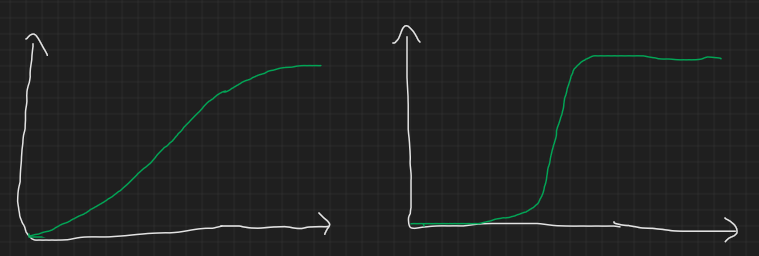
\includegraphics[width = 0.7\textwidth]{figure_man/placeholder_discrimination}
\end{center}

\end{vbframe}

% ------------------------------------------------------------------------------

\begin{vbframe}{Calibration}

\begin{itemize}
  \item \textbf{Calibration}, on the other hand, assesses the concordance of 
  predicted probabilities with the observed outcome (for any reasonable
  grouping). \\
  \textcolor{blue}{$\rightarrow$ For scoring classifiers, evaluating 
  calibrations requires transformation of scores to posterior probabilities 
  first.}
  \item Predictions of a well-calibrated classifier follow approximately the 
  same distribution as the true data labels.
  \item Poor calibration occurs with imbalanced classes or when the learner 
  lacks a probabilistic framework (e.g., $k$-NN, trees).
  % \begin{itemize}
  %   \item The learner has no probabilistic framework in the first place (e.g.,
  %   $k$-NN or trees).
  %   \item Classes are imbalanced.
  % \end{itemize}
  \item We distinguish two different notions of calibration:
  \begin{itemize}
    \item \textbf{Calibration in the large} is a property of the 
    \textit{full} sample.\\
    $\rightarrow$ Observed class-1 frequency in full sample vs average overall 
    predicted class-1 probability.
    \item \textbf{Calibration in the small} is a property of \textit{subsets}.\\
    $\rightarrow$ Observed likelihood in subset vs average predicted class-1 
    probability in that subset.
  \end{itemize}
\end{itemize}

% We consider data with a binary outcome $y$.
% \begin{itemize}
%   \item \textbf{Calibration:} When the predicted probabilities closely agree
%     with the observed outcome (for any reasonable grouping).
%   \begin{itemize}
%     \item \textbf{Calibration in the large} is a property of the \textit{full sample}.
%     It compares the observed probability in the full sample  (e.g. proportion of observations for which $y=1$)
% <!-- (e.g., 10% if 10 of 100 individuals have the outcome being predicted, e.g. $y=1$) -->
%     with the average predicted probability in the full sample.
%     \item \textbf{Calibration in the small} is a property of \textit{subsets} of the sample.
%     It compares the observed probability in each subset with the average
%     predicted probability in that subset.
%   \end{itemize}
%   \item \textbf{Discrimination:} Ability to perfectly separate the population into $y=0$ and $y=1$.
%     Measures of discrimination are, for example, AUC, sensitivity, specificity.
% \end{itemize}

\end{vbframe}

% ------------------------------------------------------------------------------

\begin{vbframe}{Calibration and Discrimination}

%<!-- http://www.uphs.upenn.edu/dgimhsr/documents/predictionrules.sp12.pdf -->

\begin{itemize}
  \item A well-calibrated classifier can be poorly discriminating.
  \item E.g., consider two probabilistic classifiers $f_1$ and $f_2$:
  \lz
  % \begin{table}[]
  %   \centering
  %   \begin{tabular}{rrrr}
  %     \small
  %     \hline
  %     observation nr. & truth & prediction $f_1$ & prediction $f_2$ \\
  %     \hline
  %     1        & 1     & 1           & 0           \\
  %     2        & 1     & 1           & 1           \\
  %     3        & 0     & 0           & 1           \\
  %     4        & 0     & 0           & 0           \\ \hline
  %     avg. class-1 prob. & 50\%  & 50\%        & 50\%        \\
  %     \hline
  %   \end{tabular}
  % \end{table}
  \begin{table}[]
    \footnotesize
    \centering
    \begin{tabular}{rrrr}
      \hline
      observation nr. & truth & prediction $f_1$ & prediction $f_2$ \\
      \hline
      1 & 1 & 0.9 & 0.6 \\
      2 & 1 & 0.9 & 0.6 \\
      3 & 1 & 0.9 & 0.4 \\
      4 & 0 & 0.1 & 0.4 \\
      5 & 0 & 0.1 & 0.4 \\
      6 & 0 & 0.1 & 0.6 \\ \hline
      avg. class-1 prob. & 50\%  & 50\%  & 50\% \\
      \hline
    \end{tabular}
  \end{table}
  \lz
  \item Both classifiers have identical calibration in the large (50\%), 
  but clearly, $f_1$ has better discriminative power.
\end{itemize}

% <<eval = FALSE, echo = FALSE>>=
% truth = c(1,1,0,0,0,0)
% pred.rule.1 = c(1,1,0,0,0,0)
% pred.rule.2 = c(0,0,0,0,1,1)
% kable(data.frame(truth = truth, "pred rule 1" = pred.rule.1, "pred rule 2" = pred.rule.2))
% @

\framebreak

\begin{itemize}
  \item Likewise, a well-discriminating classifier can have bad calibration:
  \lz
  \begin{table}[]
    \footnotesize
    % \centering
    \begin{tabular}{rrrr}
      \hline
      observation nr. & truth & prediction $f_1$ & prediction $f_2$ \\
      \hline
      1 & 1 & 0.97 & 0.99 \\
      2 & 1 & 0.97 & 0.99 \\
      3 & 0 & 0.01 & 0.67 \\
      4 & 0 & 0.01 & 0.67 \\
      5 & 0 & 0.01 & 0.67 \\
      6 & 0 & 0.01 & 0.67 \\
      7 & 0 & 0.01 & 0.67 \\
      8 & 0 & 0.01 & 0.67 \\ \hline
      avg. class-1 prob. & 25\%  & 25\%  & 75\% \\
      \hline
    \end{tabular}
  \end{table}
  % \begin{table}[]
  % \centering
  % \begin{tabular}{rrrr}
  % \hline
  % observation nr. & truth & prediction $f_1$ & prediction $f_2$ \\
  % \hline
  % 1        & 1     & 0.9           & 0.9         \\
  % 2        & 1     & 0.9           & 0.9           \\
  % 3        & 0     & 0.1          & 0.7           \\
  % 4        & 0     & 0.1         & 0.7           \\ \hline
  % avg. class-1 prob. & 50\%  & 50\%        & 80\%        \\
  % \hline
  % \end{tabular}
  % \end{table}
  \lz
  \item Both classifiers discriminate well (e.g., setting thresholds at
  $\theta_1 = 0.5$, $\theta_2 = 0.8$).
  \item Classifier $f_2$ is, however, rather poorly calibrated: the probability 
  of class 1 would be estimated at three times the true proportion.
\end{itemize}
\end{vbframe}

% ------------------------------------------------------------------------------

\endlecture
\end{document}
